 %%%%%%%%%%%%%%%%%%%%%%%%%%%%%%%%%%%%%%%%%%%%%%%%%%%%%%%%%%%%%%%%%%%%%%%%%%%%%%%%%%
%%																				%%
%% File name: 		01sarah.tex													%%
%% Project name:	Hochleistungsantenne										%%
%% Type of work:	T3X00 project work											%%
%% Author:		Sarah Brückner, Maximilian Stiefel, Hannes Bohnengel		%%
%% Date:		27th Arpil 2016												%%
%% University:		DHBW Ravensburg Campus Friedrichshafen						%%
%% Comments:		Created in gedit with tab width = 4							%%
%%																				%%
%%%%%%%%%%%%%%%%%%%%%%%%%%%%%%%%%%%%%%%%%%%%%%%%%%%%%%%%%%%%%%%%%%%%%%%%%%%%%%%%%%

\chapter{Einführung}
\section{Amateurfunksatelliten}
Seit den sechziger Jahren sind Amateurfunker an der Raumfahrt beteiligt. Nur vier Jahre nach dem 
Start des ersten Satelliten Sputnik 1 wurde der erste Amateurfunksatellit OSCAR-1 am 12. Dezember 
1961 erfolgreich gestartet. OSCAR bedeutet Orbiting Satellite Carrying Amateur Radio und war 22 
Tage in seinem Orbit. Dabei konnten 570 Funkamateure in 28 Ländern ihre Beobachtungen zum 
OSCAR-Projekt melden.
In dieser Studienarbeit soll die Bodenstation erdnahe Satelliten verfolgen können. 
Allgemein teilt man die Satelliten in GEO, MEO, HEO und LEO Satellitenbahnen ein \cite{orbit}.
\begin{itemize}
  \item GEO (Geostationary Orbit): Umlaufbahn in 35790 km Höhe und Umlaufzeit von einem Tag. Empfangsfenster für die Bodenstation: Immer. Dazu 
gehören unter anderen die Satelliten Astra und Meteosat.
  \item MEO (Medium Earth Orbit): Umlaufbahn in 6000-36000 km Höhe und Umlaufzeit von 5-12 Stunden. Empfangsfenster für die Bodenstation: 2–4 
Stunden. Darunter fallen die Navigationssatelliten wie GPS, Galileo und GLONASS.
  \item HEO (Highly Elliptical Orbit): Umlaufbahn in 200-15.000 km bzw. 50.000-400.000 km und Umlaufzeit von $\sim 12$ Stunden. Empfangsfenster für 
die Bodenstation: 8 Stunden. Satelliten in diesem Orbit eigenen sich zur Versorgung von Polargebieten, da die geostationären Satelliten oberhalb von 
$82^\circ$ Elevation nicht mehr zu empfangen sind. Beispiele für HEO Satelliten sind AO10, AO13, AO40.
  \item LEO (Low Earth Orbit): Umlaufbahn in 200-1500 km Höhe und Umlaufzeit von 1.5-2 Stunden. Empfangsfenster für die Bodenstation: unter 15 
Minuten. Dazu gehören die Amateurfunksatelliten, welche der Satellitenkommunikation zwischen Funkamateuren und auch zu experimentellen Zwecken 
dienen, wie AO-7 und AO-51. Außerdem befindet sich die ISS auf dieser niedrigen Erdumlaufbahn.
\end{itemize}
Amateurfunksatelliten kommunizieren im 2-Meter- und 70-Zentimeterband \cite{Wiki:amateur} und ermöglichen einen 
internationalen Sprech- und Datenfunk. Außerdem senden diese Satelliten
auch Messwerte der Betriebsdaten des Satelliten. Diese Satelliten werden meist von Hochschulen oder Amateurfunkvereinigungen gebaut und mit weiteren 
Satelliten an Board einer Rakete in das All geschossen. Dabei handelt es sich um kleine, leichte Satelliten, auch ``Cubesat'' genannt.

\begin{figure}[h]
 \centering
 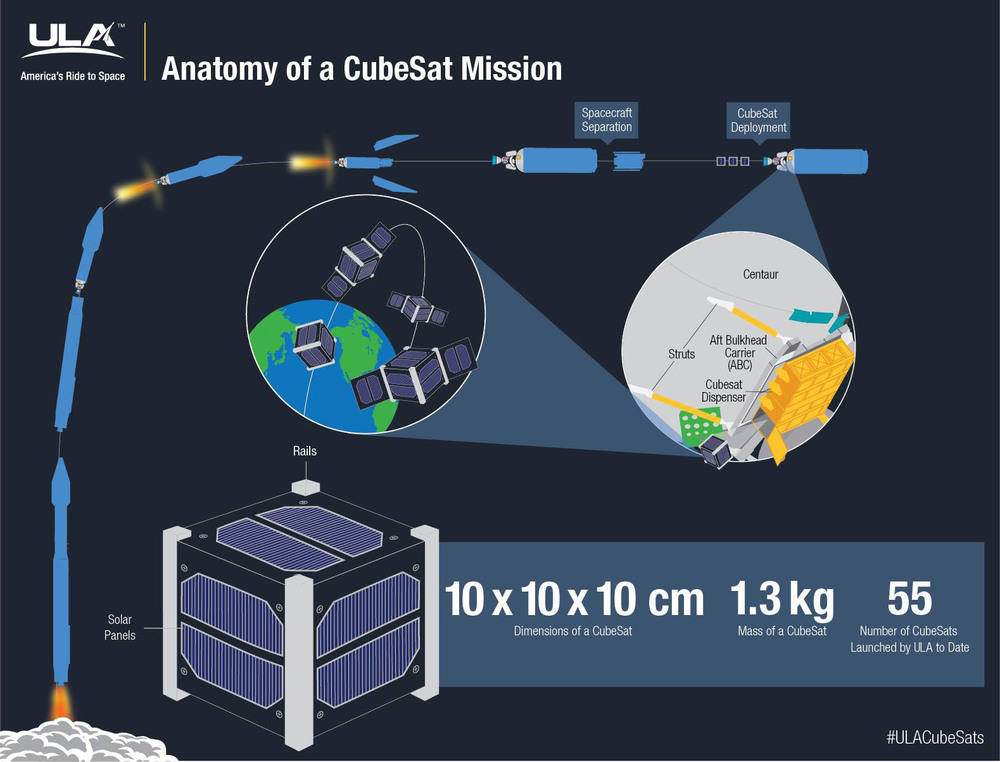
\includegraphics[width=0.7\linewidth]{./images/cubesat}
 \caption{Cubesat, Quelle: \cite{cubesat}}
 \label{fig:cubesat}
\end{figure}
Die Grafik \ref{fig:cubesat} zeigt einen beispielhaften Cubesat und wie dieser von einer Rakete in 
das All geschossen wird. Im Vergleich, der ASTRA 1L Satellit mit 
einer Spannweite von 20 Meter und einem Gewicht von 4,5 Tonnen. Erdnahe Satelliten umkreisen die 
Erde ständig und haben daher nur ein beschränktes 
Zeitfenster, in dem man mit einem solchen Satelliten arbeiten kann. Davor befindet sich der Satellit durch die Erdkrümmung hinter dem Horizont und 
ist daher unerreichbar. Daher ist es für die Bodenstation wichtig zu wissen wann der Satellit am Horizont auftaucht um die Antenne in die richtige 
Position nach zuführen. Nach der korrekten Nachführung folgt die Kontaktaufnahme. Dafür besitzt jeder Satellit einen Transponder um Daten zu 
empfangen und wieder abzustrahlen. In der folgenden Tabelle sind die Transpodermodi der Amateurfunksatelliten gelistet. 
\begin{table}[h]
	\centering
	\caption[Abkürzungen der Transpondermodi]{Abkürzungen der Transpondermodi, Quelle: \cite{amateursat}}
	\begin{tabular}{c|l}
		Bezeichnung & Band\\ 
		V & 2-m-Band 	\\
		U & 70-cm-Band 	\\
		L & 23-cm-Band 	\\
		S & 13-cm-Band 	\\
		X & 3-cm-Band 	\\
	\end{tabular} 
	\label{tab:modi}
\end{table}

Der Modus gibt an, in welchem Frequenzbereich der Satellit hört und auf welchem er sendet. Ein Transponder in dem 
Modus VU empfängt im 2-m-Band und sendet im 70-cm-Band. Ein Signal, das der Satellit zur Erde schickt nennt man ``Downlink'' und von der Basisstation 
zum Satelliten ``Uplink''.
Historisch wurden die Uplink- und Downlink- Bänder mit folgenden Buchstaben codiert: Modus A,B oder J.
Das für diese Studienarbeit verwendete Funkgerät IC-9100 kann in den Modi B und J arbeiten \cite[S.153]{radiomanual}
\begin{itemize}
 \item Mode B: Uplink: 70 cm - Downlink:  2  m 
 \item Mode J: Uplink:  2  m - Downlink: 70 cm
\end{itemize}
Einige Cubesats senden in \ac{CW} das Rufzeichen sowie ihre Telemetriedaten aus und dienen der Funktionskontrolle.
Um Informationen zu empfangen oder zu senden, gibt es einige Möglichkeiten im Amateurfunk. Es werden im Folgenden die wichtigsten Betriebsarten 
vorgestellt. 
\begin{itemize}
 \item SSB -- Single Side Band: Eine von den Amateurfunkern eingeführten Betriebsart für das Fernsprechen. Diese ist eine leistungsfährigere und 
effizientere Weiterentwicklung der Amplitudenmodulation. Bei der Amplitudenmodulation werden zwei Seitenbänder mit den Informationen und ein Träger 
benötigt. Daher ist ein AM-Signal sehr breit und störanfällig. Anders bei der SSB Betriebsart. Hier wird auf den Träger und dem zweiten Seitenband 
verzichtet. Trotz dessen kann ein gutes Sprachsignal übertragen werden.  
 \item FM -- Frequenzmodulation: Bei der Frequenzmodulation wird die Information in eine Frequenz gepackt und die Amplitude bleibt dabei 
konstant. FM ermöglicht eine qualitativ gute, störungsfreie Übertragung von Sprache.   
 \item Packet Radio -- Datenübertragung: Diese Betriebsart überträgt digitale Daten in dem kurze Datenpackete ausgesendet werden und am Emfänger 
wieder zusammen gesetzt werden. Dadurch können Funkamateure mit ihren üblichen UKW-Funkgeräten untereinander Daten austauschen. Für die Kommunikation 
zwischen Amateurfunksatelliten und den Bodenstationen wird vorwiegend das Packet-Radio-Protokoll mit FSK-Modulation (Frequenzumtastung) verwendet.
\end{itemize}

\newpage
Die 1969 gegründete Organisation AMSAT ist eine Vereinigung von Funkamateuren, welche Raumfahrtsatelliten entwickeln und kostengünstige 
Raumfahrtmissionen realisieren. Unter anderem dokumentiert AMSAT auch alle Amateurfunksatelliten und deren Status. 
\begin{figure}[h]
 \centering
 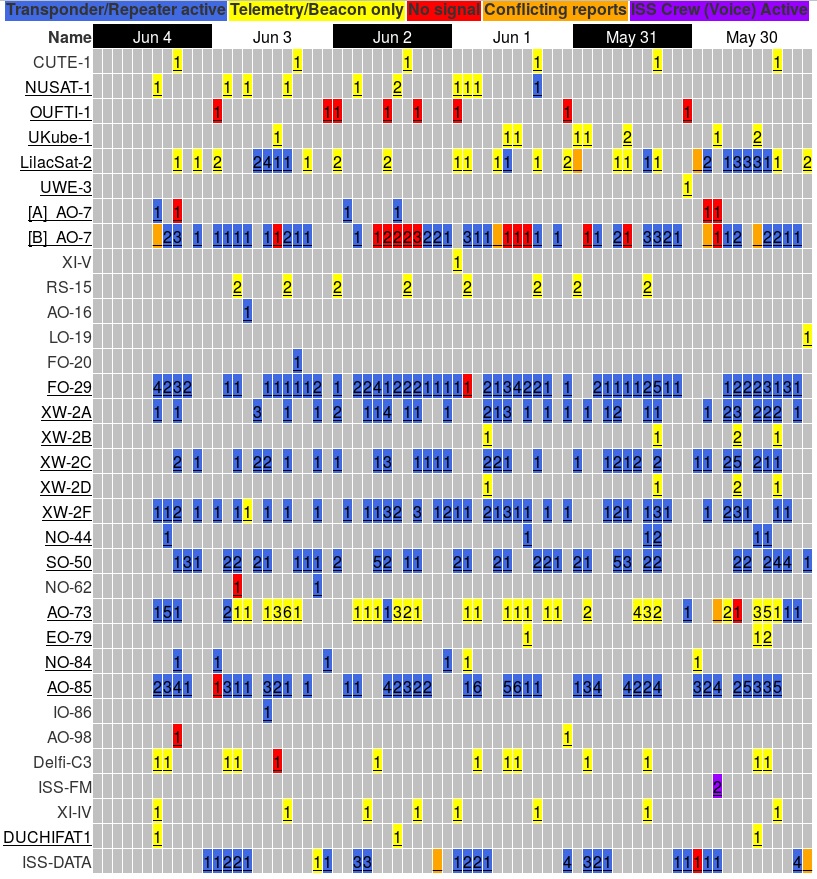
\includegraphics[width=0.65\linewidth]{./images/amsatlist}
 \caption{AMSAT Live OSCAR Satellite Status, Quelle: \cite{amsat}}
 \label{fig:amsat}
\end{figure}
In der Grafik \ref{fig:amsat} sind die Satelliten mit dem aktuellen Statusbericht (04. Juni 2016) gelistet. Diejenigen Satelliten mit blauer 
Markierung sind aktiv, wohingegen die roten Satelliten kein Signal zu dem jeweiligen Zeitpunkt von sich gegeben haben. Gelb bedeutet, dass nur die 
Telemetriedaten empfangen wurden und orange, dass Konflikte bestehen. Für die Studienarbeit sind diese Informationen sehr nützlich, um Satelliten 
tracken zu verfolgen. 
%betriebsarten
%http://www.hobbyfunk.de/cb/betriebsarten.html
%http://www.ov-lennestadt.de/amateurfunk/auf-ultrakurzwelle